\section{Network Scenario and Modeling}

\begin{figure}[h!]
  \centering
    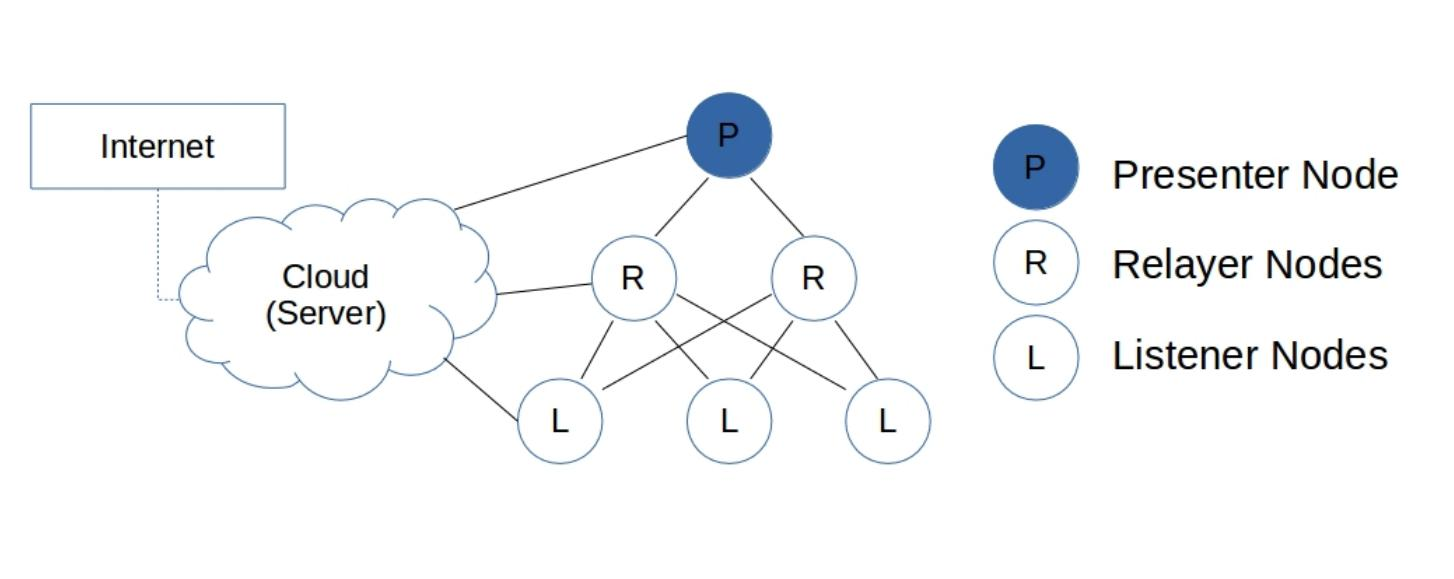
\includegraphics[width=0.5\textwidth]{figures/model1_test2.jpg}
  \caption{P2P-based Model for VoIP}
  %\vspace{-1in}
  \label{fig:mod1}
\end{figure}
There are four main types of components/nodes in the designed scenario, a
presenter, multiple relayers and listeners, and a remote cloud server.
In our application all the nodes are connected with the cloud server and
they do not need any kind of internet connection for transmitting voice through the network.
Each component can coordinate with one another in order to stream content such
as the voice or camera videos of the speaker, to the listeners in real-time. As
shown in Fig.~\ref{fig:mod1}, the network is organized in a hierarchical
architecture. The presenter will produce the streaming content from the
root node and broadcast it to the relayers and listeners, as well as to
the cloud servers for backup.

For example, one can think of the model as a lecture in real life. A presenter
is an instructor who gives the lecture in front of the room, and the
listeners are
students who are listening the lecture (can also be remote listening). When
a
presenter creates a presentation, the voice or videos being recorded will be
sent to both the child nodes and the remote cloud server so that the servers can
maintain a full copy for the streaming content in the presentation. All the
other nodes can passively receive the packets from the presenter.
%The relayers and cloud server are possible approaches the instructor adopts to
%pass on that voice stream.
%How well a student understand is not a good
%predictor of instructor’s capability; it largely depends on the media, that
%is, how well the instructor could transfer his thinking in a explanatory way.
%And that is where the cloud and relayers come into play.
There are different routes a voice packet can travel through. The
listeners receive voice packets through the relayers while the cloud server
can provide back-up services. If any of the listeners or relayers encounter a
data loss due to a bad network condition, the node can send requests to the
cloud server and retrieve the missing content. Once a relayer goes down,
the listeners will request the voice stream from the cloud. Presumably the
relayer will rejoin, and the system will reorganize to optimize in that case.
It is presumed that relayers are closer to the listeners, affording better
service due to locality and load distribution. The cloud will take
over
and serve as the main approach to deliver packets.
%Noted that only in simple cases where all attendees share the same role do
%relayers act as routers.
For a more complex scenario, where there are multiple roles for the listeners,
relayers act as filter and only forward packets to the designated attendees.

\begin{figure}[h!]
  \centering
      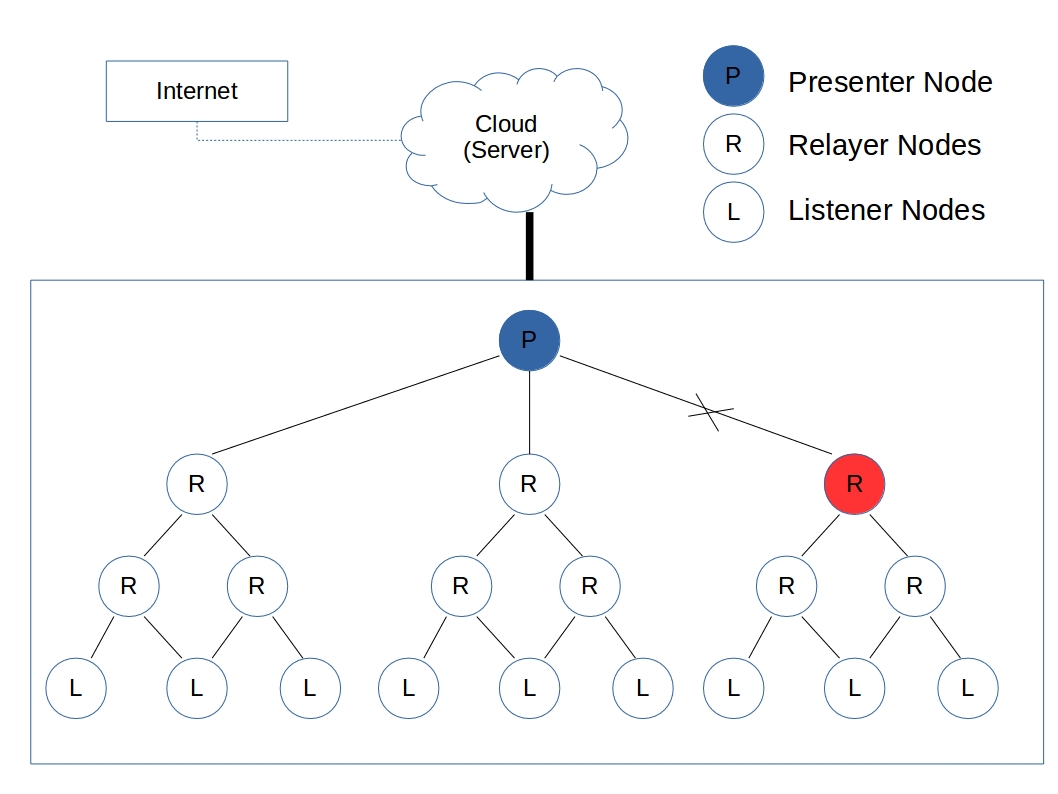
\includegraphics[width=0.5\textwidth]{figures/model2_test2.jpg}
  \caption{Relayers Become Presenters}
  \label{fig:mod2}
\end{figure}

However, this simple hierarchical architecture cannot be adaptable to
dynamic network changes and could experience an unbalanced network
traffic problem which could seriously reduce the quality of service and
experience. For example, Fig.~\ref{fig:mod2} shows that if a
high-level (near to the root) relayer suddenly leaves the network, all the
nodes lower than the relayer will not be able to receive the streaming content
any more, and thus the server will receive a large quantity of requests from the
nodes which results in lossing the connection from the presenter. This will cause the server
bandwidth to be occupied by these nodes which will make the network flow
unbalanced. Also, the relayers among these nodes could lose their advantage in
passing the content to the listeners, as the listeners can already obtain the
requested packets from the cloud server and the bandwidth between the relayers
and the listeners is wasted.

Therefore, our proposed solution is to design a P2P-based
architecture among the relayers
and listeners. The server could act as the tracker in this scenario. Every node
will have to register with the server first when it joins in a presentation so
that the server will be aware of the network situation for each node. According
to the information the server receives from each node (including bandwith,
account information based on the future business model, etc.), some nodes will
be selected as relayers at different levels, while the other nodes will act as
the listeners (leaves) and establish connections with the relayers. The nodes
at the same level will be connected as well, to establish the P2P-based
architecture, as shown in Fig.~\ref{fig:mod3}.


\begin{figure}[h!]
  \centering
      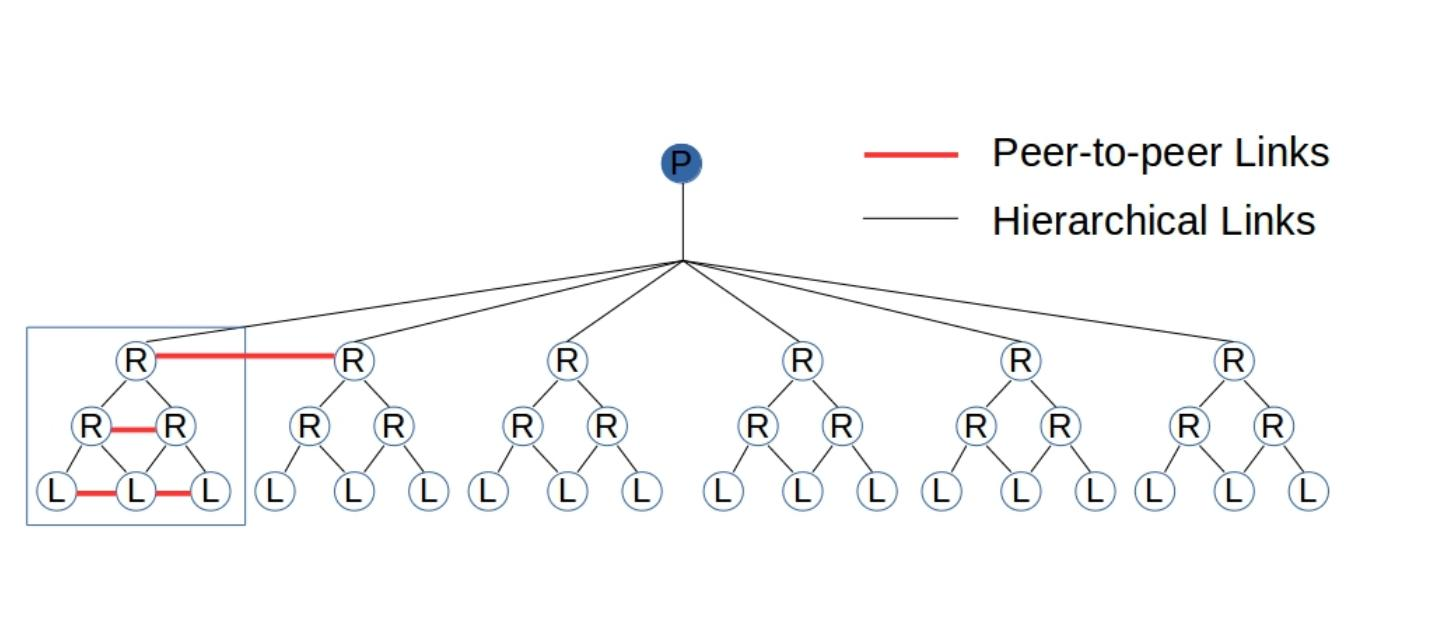
\includegraphics[width=0.5\textwidth]{figures/model3_test2.jpg}
  \caption{Relayers Become Presenters}
  \label{fig:mod3}
  \vspace{-0.15in}
\end{figure}


\begin{comment}
Besides, the concept of background channel will be applied for transmitting the
data in the background. Apart from the live channel which ensures the client to
have the presentation on live, there will also be a background channel to help
to upload or download previous missing data that make the data of the
presentation synchronized and completed in both server and client side while the
clients won’t even notice.
\end{comment}







